\documentclass{article}

\usepackage{url} 

\usepackage{pdfpages}
\usepackage{lastpage}
\usepackage{fancyhdr}
\usepackage{ngerman}
\usepackage{listings}

\usepackage{tabularx}
\usepackage{floatrow}
\usepackage[tableposition=top]{caption}
\floatsetup[table]{capposition=top}

\usepackage{amsmath, amssymb}

\usepackage[utf8]{inputenc}


\usepackage[numbib]{tocbibind}



\newcommand\twodigits[1]{%
   \ifnum#1<10 0#1\else #1\fi
}



\lhead{Abbe-Theorie}
\rhead{13. November 2020\\T. Maier, J. Winkler}
%\cfoot{\twodigits{\thepage}~/ \pageref{LastPage}}
\cfoot{{\thepage}~/ \pageref{LastPage}}

\newcommand{\W}{\text{W}}
\newcommand{\V}{\text{V}}
\newcommand{\A}{\text{A}}


\newcommand{\mini}{\operatorname{min}}


\begin{document}

\parindent0cm

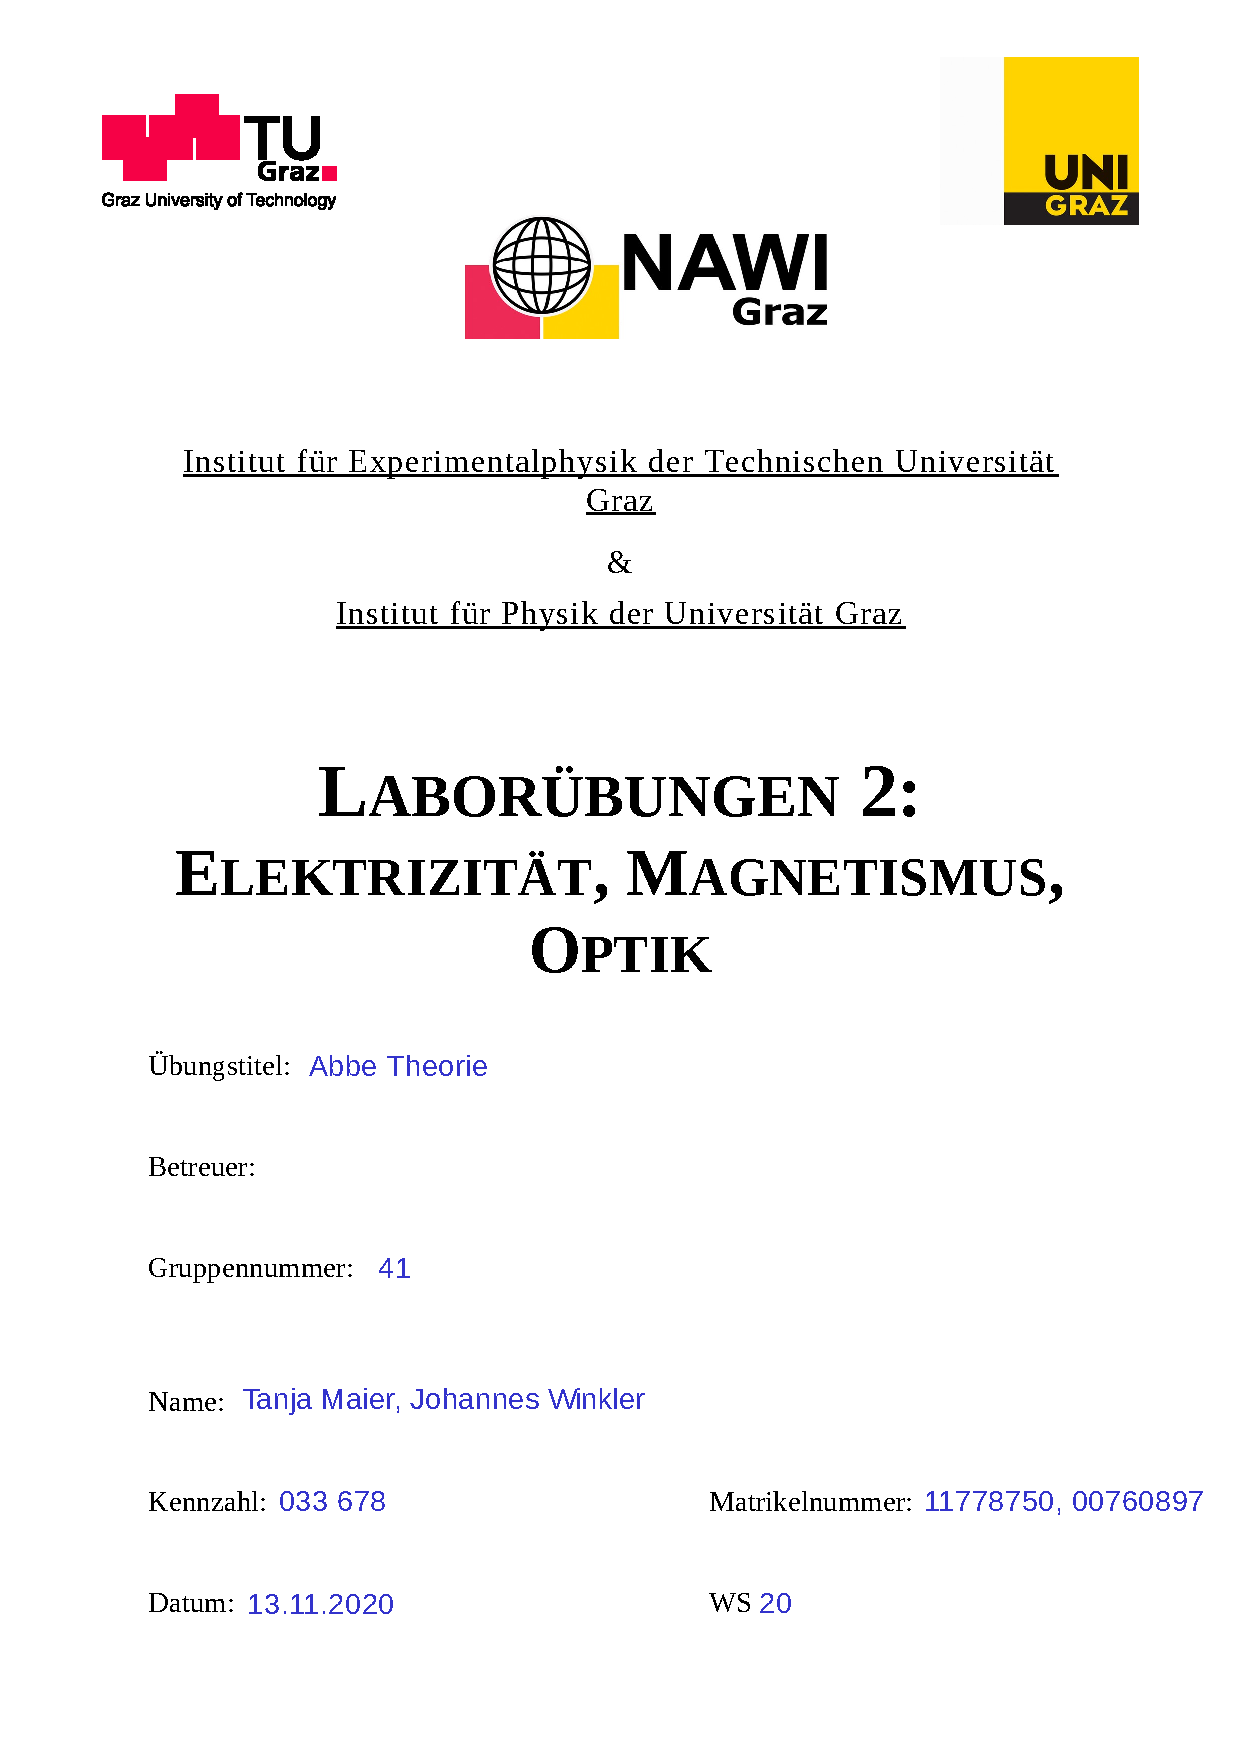
\includepdf{Deckblatt.pdf}


\pagestyle{fancy}

\tableofcontents
\newpage


\section{Aufgabenstellung}

\begin{enumerate}
\item Qualitative  Untersuchung des Zusammenhangs zwischen der  Auflösung  des  Bildes  eines Spaltgitters (Testobjekt) und der Anzahl der transmittierten Beugungsordnungen.
\item Quantitative Bestimmung  des Auflösungsvermögens  einer  Linse  in Abhängigkeit  von  ihrer numerischen Apertur ($N_A$) für zwei unterschiedliche Wellenlängen der Beleuchtung.
\end{enumerate}


\section{Voraussetzungen und Grundlagen}

Die Abbesche Theorie besagt, dass das Auflösungsvermögen eines Objekts maßgeblich durch die Wellenlänge des eingestrahlten Lichts begrenzt wird. Das Auflösungsvermögen ist dabei die Fähigkeit eines Instruments Objektdetails noch getrennt abbilden zu können. Eine der Grundlage für diese Theorie bildet das Huygenssche Prinzip, wonach jeder Punkt einer Wellenfront der Ausgangspunkt einer neuen kugelförmigen Elementarwelle ist.

Licht trifft also auf ein Gitter, es bilden sich kugelförmige Wellen und es kann sowohl konstruktive als auch destruktive Interferenz beobachtet werden. Die Abbesche Theorie sagt hier, dass jedoch mindestens die Maxima nullter und erster Ordnung von einer Linse erfasst werden müssen, um überhaupt eine Auflösung zu erhalten. Außerdem kann die Linse (rein technisch) nicht unendlich groß gebaut (d.h. es können nie alle Maxima erfasst werden) und auch nicht beliebig nahe an das Gitter herangebracht werden. Der Zusammenhang zwischen Einfallswinkel $\alpha$ des Lichts, das höchstens von der Linse erfasst werden kann und Brechzahl $n$ des Mediums, in dem sich die Apertur befindet, ist durch die sogenannte numerische Apertur $N_A$ (Auflösungvermögen des Mikroskops) gegeben
\begin{align}
N_A = n\cdot\sin(\alpha)
\end{align}
Betrachtet man nun zwei Punkte eines Gitters, die im Abstand $x$ voneinander entfernt sind und ebenfalls jeweils eine kugelförmige Welle aussenden, so ergibt sich der Zusammenhang
\begin{align}
\sin(\alpha) = \frac{\lambda}{x\cdot n}
\end{align}
bzw. durch Umformung
\begin{align}
x = \frac{\lambda}{n\cdot \sin(\alpha)} = \frac{\lambda}{N_A} 
\end{align}
wobei $\alpha$ hier dem Winkel zwischen nullter und erster Ordnung der Maxima und $\lambda$ der Wellenlänge des eingestrahlten Lichts entspricht.


Der kleinstmögliche Abstand $x_{\operatorname{min}}$ ist dann gegeben durch
\begin{align}
x_{\text{min}} = 0.61 \cdot \frac{\lambda}{N_A}
\end{align}
Außerdem kann für $r<<f$ und $n=1$ (also Luft bzw Vakuum) angenommen werden, dass
\begin{align}
N_A \approx r/f
\end{align}
wobei $f$ der Abstand zwischen Linse und Blende und $r$ der Radius der Lochblende ist.  (vgl. \cite{quelle1} \cite{quelle2} \cite{quelle3})

Zum ähnlichen Überlegungen kommt man aufgrund des Rayleigh-Kriteriums zur optischen Mikroskopie, welches besagt, dass zwei Punkte im Abstand $x$ gerade dann noch auflösbar sind, wenn das Beugungsscheibchen des ersten Objekts auf das erste Minimum des Beugungsscheibchens des zweiten Objekts fällt. (vgl. \cite{quelle4} \cite{quelle5})
\begin{align}
x = \frac{\frac{1.22}{2}\cdot \lambda}{N_A}
\end{align}

%\begin{figure}[H]
%\caption{Transformator}
%\label{fig:transformator}
%{\centering
%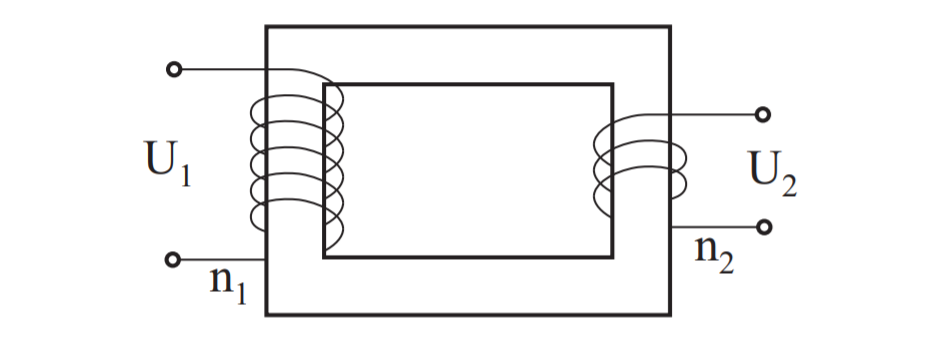
\includegraphics[scale=0.4]{transformator.png}
%~
%}
%\end{figure}





\section{Geräteliste}

\begin{table}[H]
\caption{Liste der verwendeten Geräte}

~

\begin{tabular}{l|p{3cm}p{3cm}llll}
Abk. & Bezeichnung  & Typ & Gerätenummer & Unsicherheit \\
\hline
LA & Diodenge\-pumpter Festkörperlaser THOR-Labs  & Festkörperlaser $\lambda~=~531.9~$nm & LDS5 & $\Delta \lambda = 0.05~$nm \\
\hline
RL & Rote LED &  $\lambda=470~$nm & & $\Delta \lambda = 0.05~$nm \\
\hline
BL & Blaue LED &  $\lambda=635~$nm & & $\Delta \lambda = 0.05~$nm \\
\hline
TO & Testobjekt & 1951 USAF Target  \\
\hline
L1 & Abbildungslinse 1 & $f_1 = 200~$mm & & $\Delta f_1 = 1~$mm \\
\hline
L2 & Abbildungslinse 2 & $f_2= 60~$mm, freier Durchmesser: $21.4$ mm, achromatisches Linsenpaar & & $\Delta f_2 = 1~$mm\\
\hline
L3 & Hilfslinse & $f_3 = 50~$mm, klappbar & & $\Delta f_3 = 1~$mm \\
\hline
B & Lochblenden und Irisblende & $d_1=2~$mm ~ ~ ~ ~ $d_2=3~$mm   ~~~~~~~~~~~~ $d_3=6~$mm & &  $\Delta d = 0.1~$mm \\
\hline
F & Filterrad für LEDs & \\
\hline
K & Kamera
\end{tabular}

\end{table}



\section{Beschreibung der Versuchsanordnung}


\begin{figure}[H]
\caption{Das verwendete Testobjekt, USAF 1951. aus \cite{quelle6}}
\label{fig:usaf}
{\centering
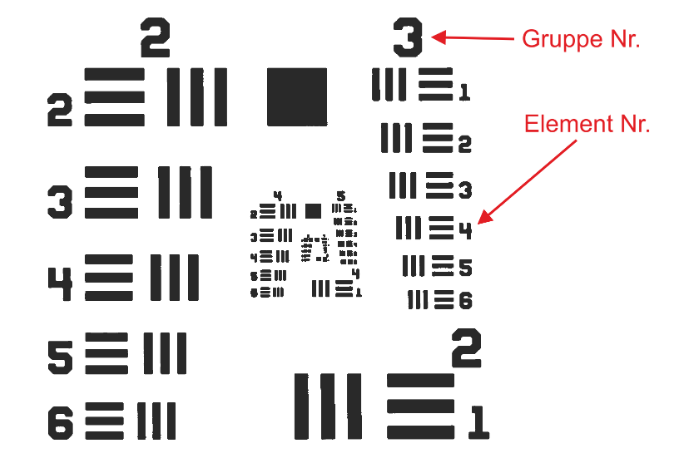
\includegraphics[scale=1.5]{usaf.png}
~
}
\end{figure}


Als darzustellendes Objekt wird Grafik \ref{fig:usaf} verwendet. Diese dient zur Bestimmung des Auflösevermögens von optischen Geräten. Es gibt mehrere Gruppen, die jeweils 6 Elemente haben. Ein Element besteht jeweils aus 3 horizontalen und 3 vertikalen Linien. Die Auflösung kann dadurch bestimmt werden, dass man die entsprechende Gruppe und das entsprechende Element angibt, mit einem / getrennt. Das Auflösevermögen wird durch jenes Element (bzw. Gruppe) bestimmt, dass am kleinsten ist und wo man trotzdem noch die horizontalen von den vertikalen Linien unterscheiden kann. Das Auflösevermögen kann in Tabelle \ref{tab:aufl} abgelesen werden.




\begin{table}[H]
\caption{Auflösungsvermögen je nach nach Element und Gruppe mit der Einheit mm$^{-1}$.}
\label{tab:aufl}
\begin{tabular}{|l||l|l|l|l|l|l|l|l|l|l|l|}
\hline
\textbf{Elem. Nr.} & \multicolumn{10}{|c|}{\textbf{Gruppen Nr.}}\\
\hline
& -2 & -1 & 0 & 1 & 2 & 3 & 4 & 5 & 6 & 7 \\
\hline
1 & 0.250 & 0.500 & 1.00 & 2.00 & 4.00 & 8.00 & 16.00 & 32.0 & 64.0 & 128.0 \\
\hline
2 & 0.280 & 0.561 & 1.12 & 2.24 & 4.49 & 8.98 & 17.95 & 36.0 & 71.8 & 144.0 \\
\hline
3 & 0.315 & 0.630 & 1.26 & 2.52 & 5.04 & 10.10 & 20.16 & 40.3 & 80.6 &  161.0 \\
\hline
4 & 0.353 & 0.707 & 1.41 & 2.83 & 5.66 & 11.30 & 22.62 & 45.3 & 90.5 & 181.0 \\
\hline
5 & 0.397 & 0.793 & 1.59 & 3.17 & 6.35 & 12.70 & 25.39 & 50.8 & 102.0 & 203.0 \\
\hline
6 & 0.445 & 0.891 & 1.78 & 3.56 & 7.13 & 14.30 & 28.50 & 57.0 & 114.0 & 228.0 \\
\hline
\end{tabular}
\end{table}






\begin{figure}[H]
\caption{Aufbau (inkl. Abmessungen) des Versuchs; $L_1$: $f_1= 200~$mm, $F$: Filterrad mit 2 LEDs, Graufilter und freiem Durchgang, $T$: Testobjekt; $L_2$: $f_2= 60~$mm; $B$: Filterrad mit 3 Lochblenden, einer Irisblende und einer Drahtblende, $L_3$ (einklappbar): $f_3= 50~$mm. Quelle: \cite{quelle6}}
\label{fig:usaf}
{\centering
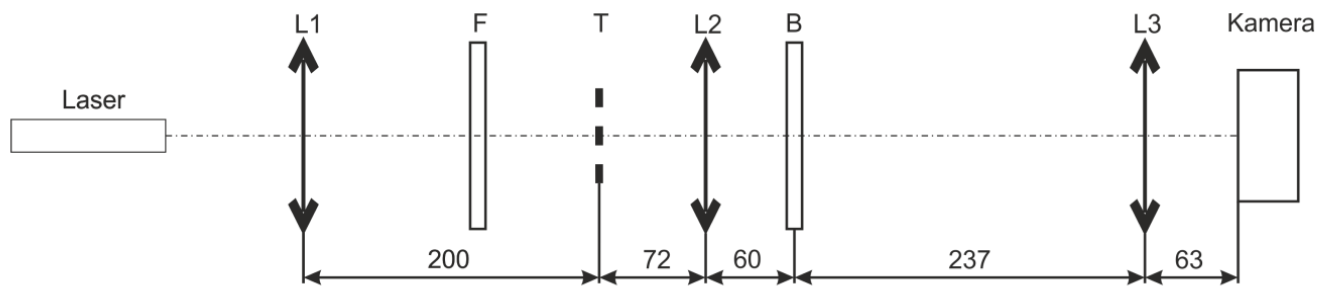
\includegraphics[scale=1]{versuch.png}
~
}
\end{figure}








\section{Versuchsdurchführung und Messwerte}

\subsection{Beugungsordnungen und Auflösung}


Zuerst wurde die geöffnete Irisblende am Filterrand $B$ in den Strahlengang gedreht und die Linse $L_3$ aus dem Strahlengang rausgeklappt. Dann wurde das Objekt scharfgestellt, indem es mit einer roten LED-Lampe beleuchtet wurde. Danach wurden die drei vertikalen Balken des 3/4 gesucht und zentriert. Anschließend wurde noch die LED-Beleuchtung durch eine Laserbeleuchtung ersetzt und das Bild des Objektes, sowie das zugehörige Beugungsbild aufgenommen (Abbildungen xy und yz).
Danach wurde mithilfe der Irisblende die Anzahl der transmittierten Ordnungen so reduziert, dass maximal die 5., die 3., die 1. oder nur die 0.Ordnung transmittiert werden. Für diese 4 Stellungen der Irisblende wurden das wieder jeweils das Bild des Objektes, sowie das zugehörige Beugungsbild aufgenommen (Abbildungen xy bis yz).
\newpage


\subsection{Auflösevermögen und Numerische Apertur}



Hier wurden beide LEDs als Lichtquellen verwendet und die numerische Apertur mit 3 Lochblenden variiert. Dann wurden jene Elemente gesucht, bei denen die horizontalen und vertikalen Balken nicht mehr unterscheidbar sind. Von den gefundenen Elementen wurden wieder die Bilder aufgenommen, sowie die eingestellten Lochblenden und die Farbe der LED-Lampe notiert (Abbildungen xy bis yz).

\newpage



\section{Auswertung}

\subsection{Beugungsordnungen und Auflösung}

Dieser Versuch läuft qualitativ ab. Hierbei zeigt sich in der Abbe-Theorie, dass in der 0. Beugungsordnung keine Information über die Struktur des Bildes übertragen wird. Um eine genauere Struktur zu erhalten, benötigt man also höhere Begungsordnungen.




\subsection{Auflösevermögen und Numerische Apertur}


Der Fehler wird nach der Größtfehlermethode berechnet und es gilt
\begin{align*}
x_b &= \frac{1}{a_{i,j}} \\
\Delta x_b &= \frac{1}{a_{i,j}^2}\cdot \Delta a_{i,j}
\end{align*}
wobei $a_{i,j}$ aus Tabelle~\ref{tab:aufl} genommen genommen wird. 


\begin{table}[H]
\caption{Gemessene Auflösungsvermögen für das blaue LED. $d$ Linsendurchmesser, $\Delta d = \pm 0.1$~mm, $E_b$ gefundenes Element für blaues Licht, $x_b$ Auflösungsvermögen vom blauen Licht (s. Tabelle \ref{tab:aufl}), $\Delta x_b$ Unsicherheit zum Auflösungsvermögen.}

\begin{tabular}{llll}
$d$ / mm & $E_b$ & $x_b$ / mm & $\Delta x_b$ / mm \\
\hline
2 & 6/1 & ... & .. \\
3 & 6/3 & ... & .. \\
6 & 7/1 & ... & .. 
\end{tabular}
\end{table}


\begin{table}[H]
\caption{Gemessene Auflösungsvermögen für das rote LED. $d$ Linsendurchmesser, $\Delta d = \pm 0.1$~mm, $E_r$ gefundenes Element für rote Licht, $x_r$ Auflösungsvermögen vom rotem Licht (s. Tabelle \ref{tab:aufl}), $\Delta x_b$ Unsicherheit zum Auflösungsvermögen.}

\begin{tabular}{llll}
$d$ / mm & $E_r$ & $x_r$ / mm & $\Delta x_r$ / mm \\
\hline
2 & 6/1 & ... & .. \\
3 & 6/3 & ... & .. \\
6 & 7/1 & ... & .. 
\end{tabular}
\end{table}






\section{Zusammenfassung und Diskussion}

Es zeigt sich hier deutlich, dass ein Zusammenhang zwischen der Schärfe des Bildes und der Anzahl der Beugungsordnungen gilt. Und zwar wird das Bild mit der Anzahl der verwendeten Beugungsordnungen schärfer.

~

Im zweiten Teil zeigt sich, dass das Bild bei rotem LED besser aufgelöst ist. Dies liegt an der höheren Wellenlänge vom roten Licht.

Zusätzlich muss auch der Durchmesser der Blende berücksichtigt werden. Bei höheren Durchmesser wird die Unsicherheit geringer. Das liegt daran, dass bei einem größeren Durchmesser mehrere Beugungsmaxima genutzt werden können.





%\newpage 
%\appendix
%\section{Python Skript}



\definecolor{commentgreen}{RGB}{2,112,10}
\definecolor{eminence}{RGB}{108,48,130}
\definecolor{weborange}{RGB}{255,165,0}
\definecolor{frenchplum}{RGB}{129,20,83}

\lstdefinelanguage{python}{
    morekeywords={def, for, range, abs, return},
    otherkeywords={<-,->, |>, \%\{, \}, \{, \, (, )},
    sensitive=true,
    morecomment=[l]{\#},
    morecomment=[n]{/*}{*/},
    morecomment=[s][\color{purple}]{:}{\ },
    morestring=[s][\color{orange}]"",
    commentstyle=\color{commentgreen},
    keywordstyle=\color{eminence},
    stringstyle=\color{red},
	basicstyle=\ttfamily,
	breaklines,
	showstringspaces=false,
	frame=tb
}
%\lstinputlisting[language=Python,captionpos=b, label=lst:test,caption={Python Skript}]{generate_numbers.py}

%\lstinputlisting[language=Python,captionpos=b, label=lst:test,caption={Bessel Auswertung}]{generate_numbers_bessel.py}


%\lstinputlisting[language=Python,captionpos=b, label=lst:test,caption={Zerstreuungslinse Auswertung}]{generate_numbers_zerstreuungslinse.py}


\begin{thebibliography}{9}
\bibitem{quelle1} \url{https://www.youtube.com/watch?v=oFJCEGcwUiQ}, 07.11.2020, 00:15 Uhr
\bibitem{quelle2} \url{https://www.spektrum.de/lexikon/physik/abbesche-theorie/13}, 07.11.2020, 00:17 Uhr
\bibitem{quelle3} \url{https://www.univie.ac.at/mikroskopie/1_grundlagen/optik/opt_instrumente/7_abbe.htm}, 07.11.2020, 00:24 Uhr
\bibitem{quelle4} \url{https://physik.cosmos-indirekt.de/Physik-Schule/Rayleigh-Kriterium}, 07.11.2020, 00:26 Uhr
\bibitem{quelle5} \url{https://www.youtube.com/watch?v=PZaUY45ce8k}, 07.11.2020, 00:27 Uhr
\bibitem{quelle6} Unterlagen aus Moodle, H. Ditlbacher, bereitgestellt von der KF Universität Graz
\end{thebibliography}


\end{document}
